\chapter{Estado del Arte}
\thispagestyle{empty}

En el campo del aprendizaje automático, el tema de la estimación de la distancia en fotografías faciales ha ganado recientemente mucha atención. Se puede observar en la Figura \ref{fig5} como van aumentando el número de publicaciones relacionadas con este tema a lo largo del tiempo, llegando a obtener un mayor número de publicaciones en 2020. Pese al aumento de publicaciones en este ámbito, es a partir del 2015 cuando se empiezan a aplicar las técnicas de deep learning. Este aumento está relacionado con los avances tecnológicos que permiten aplicar nuevas técnicas y conocimientos. 

PONER CONSULTAS DE SCOPUS (APÉNDICE O NOTA A PIE DE PÁGINA)

\begin{figure}[h]
	\centering
	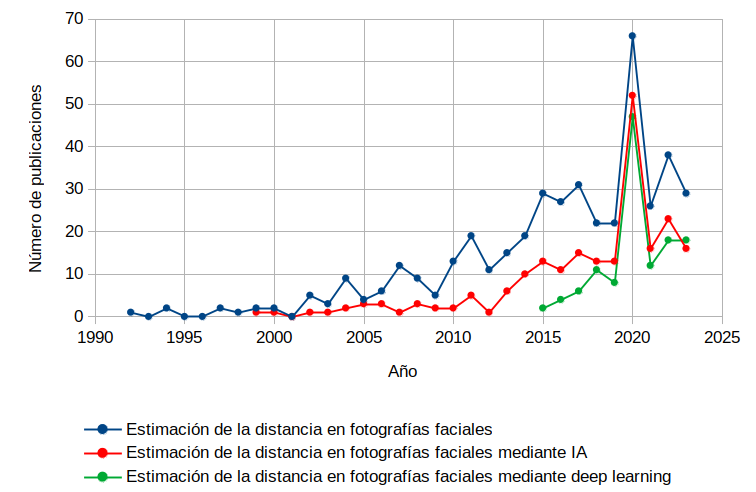
\includegraphics[scale=0.5]{imagenes/cap3/grafica_scopus3.png}
	\caption{Número de publicaciones, en Scopus, relacionadas con la estimación de la distancia en fotografías faciales en función del año de publicación}
	\label{fig5}
\end{figure}

\section{Estado del arte de la estimación del SCD en fotografías faciales}

\subsection{title}

\subsection{PerspectiveX}

\subsection{FacialSCDnet}
































218 hay TITLE-ABS-KEY ( ( deep AND learning ) OR ( machine AND learning ) OR ( artificial AND intelligence ) OR ( computer AND vision ) OR ( soft AND computing ) AND ( ( distance OR depth ) AND estimation AND ( photographs OR images ) AND facial ) ) AND ( LIMIT-TO ( SUBJAREA , "COMP" ) OR LIMIT-TO ( SUBJAREA , "ENGI" ) )
y con solo deep learning 126
y sin deep learning 430
y sin facial 6,458 

1. Van Dijk, T.,  De Croon, G. (2019). How do neural networks see depth in single images? In IEEE/CVF international conference on computer vision (pp. 2183–2191).
